
%%%%%%%%%%%%%%%%%%%%%%% file typeinst.tex %%%%%%%%%%%%%%%%%%%%%%%%%
%
% This is the LaTeX source for the instructions to authors using
% the LaTeX document class 'llncs.cls' for contributions to
% the Lecture Notes in Computer Sciences series.
% http://www.springer.com/lncs       Springer Heidelberg 2006/05/04
%
% It may be used as a template for your own input - copy it
% to a new file with a new name and use it as the basis
% for your article.
%
% NB: the document class 'llncs' has its own and detailed documentation, see
% ftp://ftp.springer.de/data/pubftp/pub/tex/latex/llncs/latex2e/llncsdoc.pdf
%
%%%%%%%%%%%%%%%%%%%%%%%%%%%%%%%%%%%%%%%%%%%%%%%%%%%%%%%%%%%%%%%%%%%


\documentclass[runningheads,a4paper]{llncs}

\usepackage{amssymb}
\setcounter{tocdepth}{3}
\usepackage{graphicx}
\usepackage{booktabs}
\usepackage{float}
\usepackage{url}
\urldef{\mailsa}\path|{rafael.possas, ying.zhou}@sydney.edu.au|    
\newcommand{\keywords}[1]{\par\addvspace\baselineskip
\noindent\keywordname\enspace\ignorespaces#1}

\begin{document}

\mainmatter  % start of an individual contribution

% first the title is needed
\title{Effectiveness of adversarial examples on class-imbalanced Convolutional Neural Networks}

% a short form should be given in case it is too long for the running head

% the name(s) of the author(s) follow(s) next
%
% NB: Chinese authors should write their first names(s) in front of
% their surnames. This ensures that the names appear correctly in
% the running heads and the author index.
%
\author{Rafael Possas, Ying Zhou}
%
\authorrunning{Lecture Notes in Computer Science: Authors' Instructions}
% (feature abused for this document to repeat the title also on left hand pages)

% the affiliations are given next; don't give your e-mail address
% unless you accept that it will be published
\institute{University Of Sydney, Camperdown, NSW \\
\mailsa\\
\url{https://sydney.edu.au}}

%
% NB: a more complex sample for affiliations and the mapping to the
% corresponding authors can be found in the file "llncs.dem"
% (search for the string "\mainmatter" where a contribution starts).
% "llncs.dem" accompanies the document class "llncs.cls".
%

\toctitle{Lecture Notes in Computer Science}
\tocauthor{Authors' Instructions}
\maketitle


\begin{abstract}
Image recognition and machine learning have been one of the most fast paced fields of Artificial Intelligence. A considerable amount of literature was published on the performance of Convolutional Neural Networks and the field has evolved considerably in the last years. However, as most machine learning methods, these networks suffer from the data imbalance problem. When the underlying training dataset is comprised of unequal number of samples for each label/class. Such difference naturally causes a phenomenon known as domain shift, which can be explained by the low generalisation capabilities of a model when presented with previously unseen data. Recent research have focused on a technique called Gradient Sign that forces domain shift on deep networks by creating adversarial examples. These are usually comprised of small directed changes on original data points that causes inputs to be misclassified by the predictive algorithm. Recent developments in such methods have heightened the need for better of understanding of this phenomena. This study focuses on an experimental approach that sheds light on the link between the imbalanced learning problem and adversarial examples. Through a series of experiments we try to find intuitive explanations behind the success of gradient sign methods and we evaluate their effectiveness against models trained on imbalanced datasets
\keywords{convolutional neural networks, adversarial examples, gradient sign, imbalanced training
the abstract section}
\end{abstract}


\section{Motivation}

Convolutional Networks are a class of deep learning algorithms that can use many layers of nonlinear or linear processing in cascade for feature extraction and transformation. They are still very similar to ordinary Neural Networks (made up of neurons that have learnable weights and biases). However, such algorithms makes the explicit assumption that the inputs are images and, therefore, are based on learning abstract representations of data with spatial properties \cite{canziani2016analysis}. 

Until recently, these networks were known for having high generalisation capabilities, however, methods using the internal model information were proven to successfully reduce their performance by creating inputs known as Adversarial Examples \cite{goodfellow2014}.

Adversaries can successfully force domain shift in such a way that the model becomes unable to generalise well on perturbed samples. Since training data in most circumstances can not cover the entire feature space, the real decision boundary of a classification model generally becomes more complex as the phenomenon becomes more nuanced and the feature and dimension space becomes larger \cite{goodfellow2016_book}. This can be exploited by adversaries through the use of the model error as a guideline for perturbing a sample that can successfully cause a misclassification of the input by the targeted system.

Besides the near human performance of deep convolutional neural networks, adversaries are still capable of forcing domain shift on classes with overlapping or similar distributions. This problem could then become critical when these adversaries are used to attack models where the training data has a large variance on the number of samples per class. 

\section{Related Work}

Recent work has shown that the generalisation capabilities of deep networks is rather sparse \cite{goodfellow2016}, \cite{papernot2016transf}. Thus, there is an opportunity for methods to exploit empty pockets of space and, hence, systematically create an adversary that produces an incorrect, high confidence prediction for an image without visible distortion. This can be done by adding just enough intentional noise to each pixel of the image so as to fool an algorithm into thinking that the image has an incorrect label \cite{goodfellow2014}, \cite{goodfellow2016}, \cite{papernot2016transf}, \cite{szegedy2013}. The resulting outcome of these methods are known as Adversarial Examples.

The Gradient Sign method developed by Goodfellow et al. (2014) has been used as the foundation of many of the experiments in adversarial crafting. The results have shown that DNNs can possibly have linear behavior in very high dimensional spaces.  Most inputs were miss-classified not only on Goodfellow et. al \cite{goodfellow2014}  experiments but many others \cite{billovits},\cite{goodfellow2016},\cite{papernot2016}.

Developing robustness to adversarial examples has been approached many times as academic work, recent research \cite{papernot2016} has shown that one can use transfer learning \cite{yosinski2014transferable} to perform black-box attacks against Deep Neural Networks.The combination of adversaries and transfer learning creates a threat vector for many state of the art methods. Attacks can, however, depend on some specific information of the target \cite{papernot2016transf}. As most recent applied methods depend on the network gradient information, there is a straight dependence on the network confidence per class label and the robustness of the model to adversarial attacks.

Imbalanced learning is a well known cause for lower performance of several machine learning algorithms \cite{japkowicz2002class}, \cite{krawczyk2016learning}. Data distribution on real world is often skewed and rarely contains enough information to learn all the required features of the data domain. As the dependency of specific class labels grows, the vulnerability of the system increases as wrong predictions of the critical label could lead to unwanted outcomes. Adversaries are proven to explore class distributions vicinities, and the question whether imbalanced training sets affects them is still unanswered.

This work presents an experimental approach aimed on the understanding of the factors leading to robustness to adversarial attacks on class imbalanced convolutional neural networks. Through the use of the Fast Gradient Sign Method we investigate how a skewed data distribution could affect the network resilience to such attacks. The understanding of such threat vectors is of the utmost importance for the development of current techniques, as it drives the creation of new regularisation techniques.






\section{Initial Setup}

For the purposes of this work, we aimed to use a dataset that could not only be visually rich but also could facilitate analysis between different class labels. The 2014 ImageNet dataset \cite{deng2009imagenet} would be the natural choice, however, the amount of classes would make it harder to make comparisons, as the number of classes is around 1,000. We use a dataset with similar characteristics, the CIFAR-10 \cite{krizhevsky_2009}. It contains 10 different class labels of 32x32 images, which makes it easier to train our algorithm from scratch and also to understand deeper relationships between class labels.
\subsection{Network Architecture}
In terms of network architecture, we looked into the ILSVRC competition for the highest performers.From all networks tested on Canziani et al (2016) \cite{canziani2016analysis}, the VGG16-19 from Simonyan et al. (2014) \cite{simonyan2014very}  seemed to have the best trade off between accuracy and performance (inference time). The VGG architecture won the first and second places on the ILSVRC-2014 submission on the localisation and classification task.The main contribution of the VGG network was showing that the depth of the network is a critical component for good classification performance. The model can be assembled with 16 or 19 Conv/FC layers and it features an extremely homogenous architecture that only performs 3x3 convolutions and 2x2 pooling from beginning to end.


The design of the VGG16 has been proven to work even on datasets with several classes that are very different from each other. As the dataset used in this work has only 10 classes, the two FC-4096 layers were replaced by one single layer with 512 neurons and RELU activations. In addition, the total number of convolutions blocks and pooling were reduced to 3, with the first layer having 2 stacked convolution layers followed by a max pooling of stride 2x2 and the last two layers with 3 stacked convolutions also followed by a max pooling of stride 2x2. Since CIFAR-10 images are only 32x32, the original VGG16 architecture would end up having an output of shape of only 1x1 pixel at the last layer. In order to avoid this problem, the number of layers were reduced so to fit our dataset domain
\subsection{Training Parameters}
The optimisation technique used in this work was developed by Bengio (2015) \cite{bengiormsprop}, namely RMSProp. This method is an adaptive learning rate scheme that can take the absolute values of the Hessian's eigenvalues and, therefore, approximate the equilibration pre-conditioner. As shown on Bengio's work \cite{bengiormsprop}, the method outperforms current SGD methods by achieving convergence faster.The learning rate for the method was set at $10^{-4}$ and the decay $10^{-5}$.

Our architecture was trained until no more reasonable changes  $\delta$ were detected in the validation loss so we could dismiss unnecessary training steps and consequently any kind of over-fitting. This was achieved by using the Early Stopping technique with a $\delta$ of $10^{-4}$. For instance, training would be stopped if no improvement over the specified $\delta$ was seen for 10 steps in a row.The results on the full dataset are shown on figure~\ref{fig:conf_matrix_full}.

\subsection{Gradient Sign methods}

The Gradient Sign is an exploitation of the loss function in an optimization process so one can maximize any class score for a given input image \cite{papernot2016}. Since everything in a ConvNet is differentiable it is relatively straight forward to compute the gradient information of any specific class of the input domain. Basically we choose an  output and we apply the reshaped gradient computation of that class to our input using equations 1 or 2.

Adding or subtracting noise  from images will generate different adversaries. Supposed we choose the same class gradient, adding noise $\delta$ to an image, one would be making the gradient to go "uphill" and therefore moving away from the class, this results in an increase in value of the loss function and thus should be referred as the Ascent Method. On the other hand, when moving the opposite direction (down), one would be doing a process similar to the optimization of a loss function where we approach the minimum of a function and, thus, we get closer to the desired class, this approach is hereby known as the Descent Method. When applying the perturbation we are only interested in the direction of the gradient and not its magnitude, therefore, we take the sign of the gradient and we control its magnitude through the $\epsilon$ parameter. Equations 1 and 2 are respectively for the ascent and descent perturbations described in this section.

\begin{equation}
C(x + \delta)\approx C(x) + \epsilon * sign(\nabla C)
\end{equation}
\begin{equation}
C(x + \delta)\approx C(x) - \epsilon * sign(\nabla C)
\end{equation}

Perturbations could be applied once or many times in order to successfully create an adversary. When only one iteration of perturbations is applied, we call the method FGSM (Fast Gradient Sign Method). On the other hand, applying the same perturbation many times is known as IGSM (Iterative Gradient Sign Method) \cite{goodfellow2014}. The latter could always end up into changing the classification output as it can be seen as taking small steps into the direction of our $\nabla C$. 
\subsection{Backpropagated Class Gradient}

The choice of the backpropagated class gradient has direct influence on the generated adversary. For instance, one could select a specific class as the target of a perturbation but this would ultimately introduce undesirable variance when crafting adversaries for our experiment, as each class could have different effects within our target and, thus, the perturbation could be different on each case. In order to address this problem, we have chosen the class itself as the backpropagated gradient coupled with the ascent method. The intuition behind this choice is that we look to increase the cost function of the target class by moving away from the current label.

For all classes, the amount of change on each pixel needed to be carefully chosen as we did not want to change an image too much to a point where it would be unrecognizable to human perception. Moreover, in order to test our networks, we needed an $\epsilon$ value that would provide only the minimum amount of perturbation to all classes so as to push most of the samples to the closest vicinity leading to a successful misclassification. From all the trials performed, the value of $\epsilon$ that seemed to fulfill our needs was 0.01. 
\begin{figure}
	\centering
	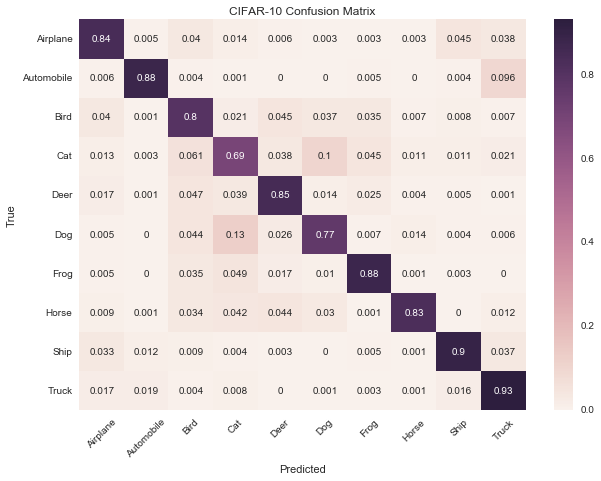
\includegraphics[height=6.5cm]{conf_matrix.png}
	\caption{Results of our adapted VGG architecture on CIFAR-10 dataset}
	\label{fig:conf_matrix_full}
\end{figure}
\subsection{Same and Different model perturbations}
Another important choice was regarding which trained network would serve as the baseline for our gradient calculation. We have generated perturbation using two different networks on each of the 10 classes. We first generate one model for each class using an undersampled and oversampled datasets. Then for each of these models we created adversaries using its own current model and the balanced network. The balanced network itself was also tested using its own adversaries on all 10 classes at once to serve as baseline for our comparison. From now on we call this same model pertubation and different model pertubation, each being subdivided into the undersample and oversample case.

\section{Results}
The objective of this research is to understand the effects of adversarial attacks on imbalanced CNNs. However, it is firstly required to create the baseline for our comparisons. This consists of creating perturbation on every class label and querying its accuracy on a fully balanced model. Canonical models assume that every object in the dataset are sampled from similar distributions. However, in real-life situations, even though the number of samples is the same, some class labels could be poorly represented by the lack of a clear structure. This could often lead to differences in the output for each specific class \cite{krawczyk2016learning}. On this way, a superficially balanced dataset does not guarantee that the model will equally generalise across all classes.
\begin{figure}
	\centering
	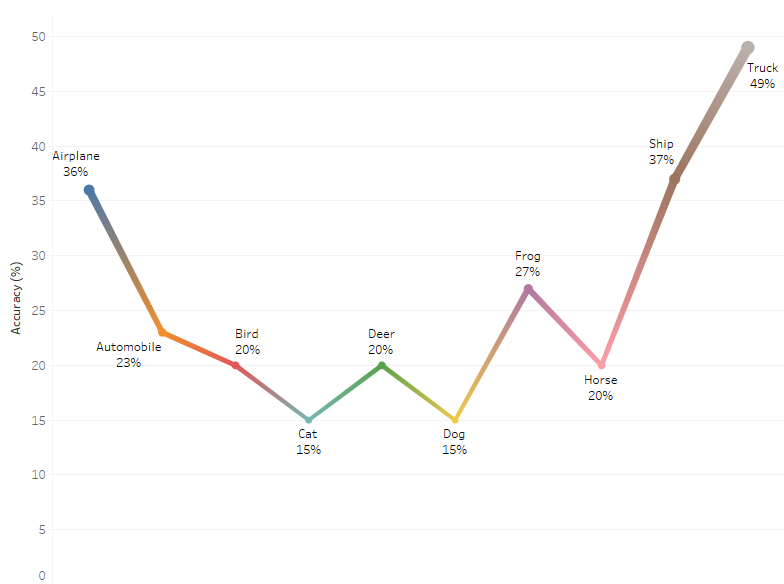
\includegraphics[height=6.5cm]{balanced_perturbed.png}
	\caption{Individual class perturbed accuracy on the balanced model}
	\label{fig:balanced_perturbed}
\end{figure}

Figure ~\ref{fig:balanced_perturbed} shows that the accuracy for all classes is drastically reduced when the balanced model is presented with adversarial examples. Even though there is enough samples for each class, the adversarial attack forces the domain shift of each individual sample towards different regions in space, causing a misclassification of the current label. The effectiveness of the adversarial attack can be partially explained by the balancing of the dataset itself. In a model where the dataset used in training aims for normalization over all classes, the network is often caught in trying to find weights and biases that generalizes well over all set of labels. Therefore, perturbations become more efficient due to a bigger proximity of classes distributions in space.
\subsection{Class under-sampling and over-sampling}
The adversarial test shows the results from two perspectives. First, on the class under-sampling with same model the accuracy for each individual class was on average 15\%, which already demonstrates higher vulnerability when compared to the balanced case. This could be explained by having the data distribution of that specific class being squished into a smaller space and, hence, decreasing the amount of perturbation required to effectively increase the cost function so as to a misclassification to happen. Therefore, the degree of the perturbation required is reduced since the class label did not explore the feature space accordingly. Second, when oversampling occurs, it is expected to have the target class expanding into space and taking as much space as possible when compared to other classes. This happens since the network performs more gradient updates on that specific class due to the amount of available samples. Perturbation on this case had a lower effect, as the small push cause by our $\epsilon$ was not enough to move points to outside of their distributions.



\begin{table}[H]
	\centering
	
	\begin{tabular}{lccccc}
		\toprule
		&\multicolumn{2}{c}{Different Model}
		&\multicolumn{3}{c}{Same Model}
		\\\cmidrule(r){2-3}\cmidrule(l){4-6}
		Class Label &Undersample &Oversample &Balanced &Undersample &Oversample \\
		\midrule
		0 - Airplane &60\%& 87\% &36\%& 19\%    & 61\% \\
		1 - Automobile &64\%& 91\% &23\%& 16\%    & 63\% \\
		2 - Bird &38\%& 73\% &20\%& 9.4\%    & 27\% \\
		3 - Cat &21\%& 72\% &11\%& 0.5\%    & 19\% \\
		4 - Deer &58\%& 80\% &20\%& 9.8\%    & 20\% \\
		5 - Dog &47\%& 76\% &15\%& 9\%    & 38\% \\
		6 - Frog &76\%& 88\% &27\%& 20\%    & 49\% \\
		7 - Horse &59\%& 88\% &20\%& 18\%    & 52\% \\
		8 - Ship &69\%& 89\% &37\%& 19\%    & 59\% \\
		9 - Truck &46\%& 87\% &49\%& 21\%    & 54\% \\
		\bottomrule	
		\hfill
	\end{tabular}
	\caption{Results for the two different sources of perturbations along with the two different imbalanced datasets}
	\label{tbl:results}
\end{table}

As the number of samples on a target class goes down, an increase of vulnerability towards that specific label is expected when compared to the balanced model. The results on table  ~\ref{tbl:results} confirms this. Networks with imbalanced datasets were more vulnerable when presented with adversarial examples. Figure ~\ref{fig:relative_difference} shows the relative difference for all the three networks (balanced, under-sampled and oversampled).  The values were calculated by finding the ratio between the new accuracy and the non-perturbed accuracy. They represent the percentage on which the initial accuracy was reduced. The under-sampled model had the higher relative difference on average, which shows that the imbalanced nature of the dataset ended-up increasing the vulnerability of the model. This poses threats to current systems as the low amount of samples during training for a specific class would  create gaps that are more easily exploited when compared to a balanced network.

\begin{figure}[H]
	\centering
	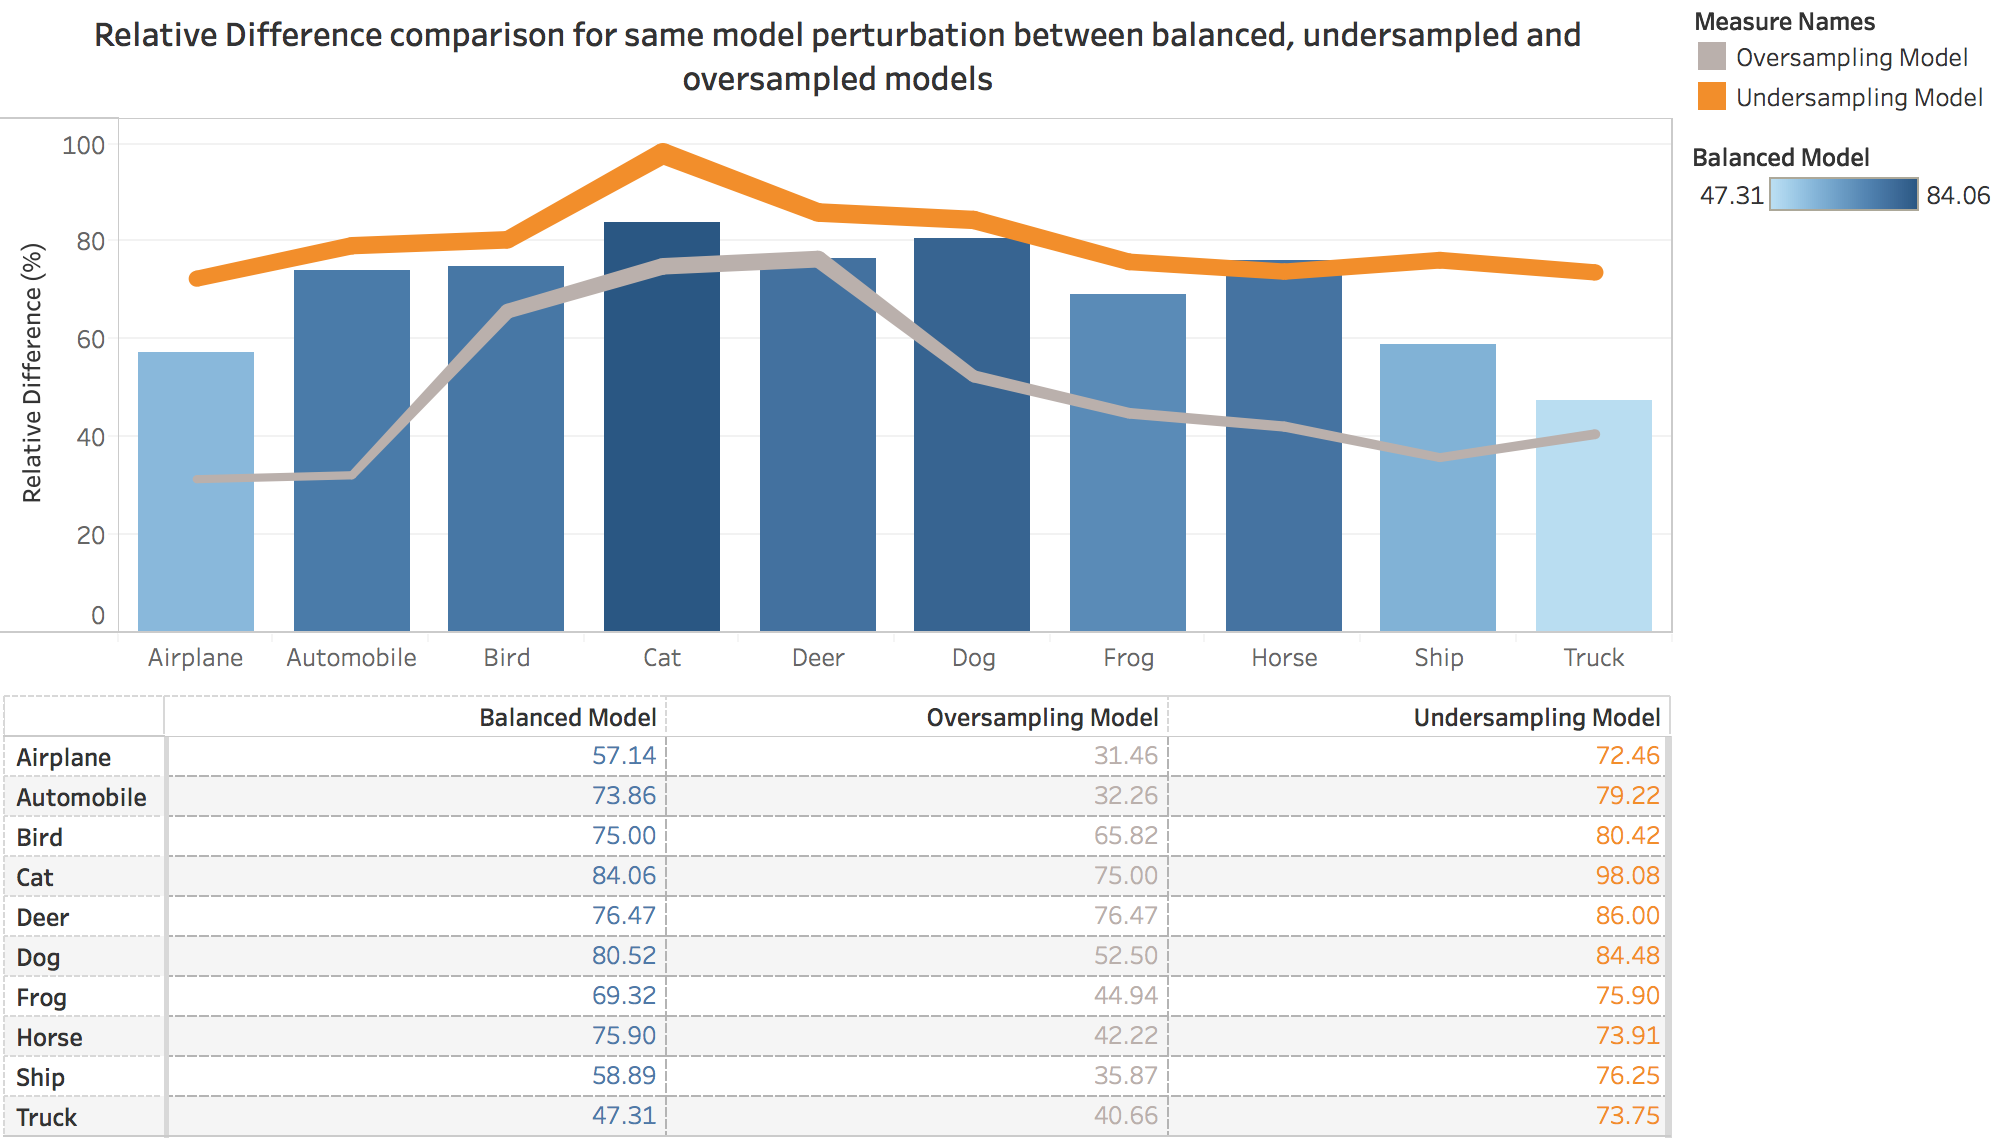
\includegraphics[height=6.5cm]{rel_diff_graph.png}
	\caption{Relative difference for each model. Higher numbers means more vulnerability}
	\label{fig:relative_difference}
\end{figure}

\subsubsection{Headings.}

Headings should be capitalized
(i.e., nouns, verbs, and all other words
except articles, prepositions, and conjunctions should be set with an
initial capital) and should,
with the exception of the title, be aligned to the left.
Words joined by a hyphen are subject to a special rule. If the first
word can stand alone, the second word should be capitalized.

Here are some examples of headings: ``Criteria to Disprove
Context-Freeness of Collage Language", ``On Correcting the Intrusion of
Tracing Non-deterministic Programs by Software", ``A User-Friendly and
Extendable Data Distribution System", ``Multi-flip Networks:
Parallelizing GenSAT", ``Self-determinations of Man".

\subsubsection{Lemmas, Propositions, and Theorems.}

The numbers accorded to lemmas, propositions, and theorems, etc. should
appear in consecutive order, starting with Lemma 1, and not, for
example, with Lemma 11.

\subsection{Figures}

For \LaTeX\ users, we recommend using the \emph{graphics} or \emph{graphicx}
package and the \verb+\includegraphics+ command.

Please check that the lines in line drawings are not
interrupted and are of a constant width. Grids and details within the
figures must be clearly legible and may not be written one on top of
the other. Line drawings should have a resolution of at least 800 dpi
(preferably 1200 dpi). The lettering in figures should have a height of
2~mm (10-point type). Figures should be numbered and should have a
caption which should always be positioned \emph{under} the figures, in
contrast to the caption belonging to a table, which should always appear
\emph{above} the table; this is simply achieved as matter of sequence in
your source.

Please center the figures or your tabular material by using the \verb+\centering+
declaration. Short captions are centered by default between the margins
and typeset in 9-point type (Fig.~\ref{fig:example} shows an example).
The distance between text and figure is preset to be about 8~mm, the
distance between figure and caption about 6~mm.

To ensure that the reproduction of your illustrations is of a reasonable
quality, we advise against the use of shading. The contrast should be as
pronounced as possible.

If screenshots are necessary, please make sure that you are happy with
the print quality before you send the files.
\begin{figure}
\centering
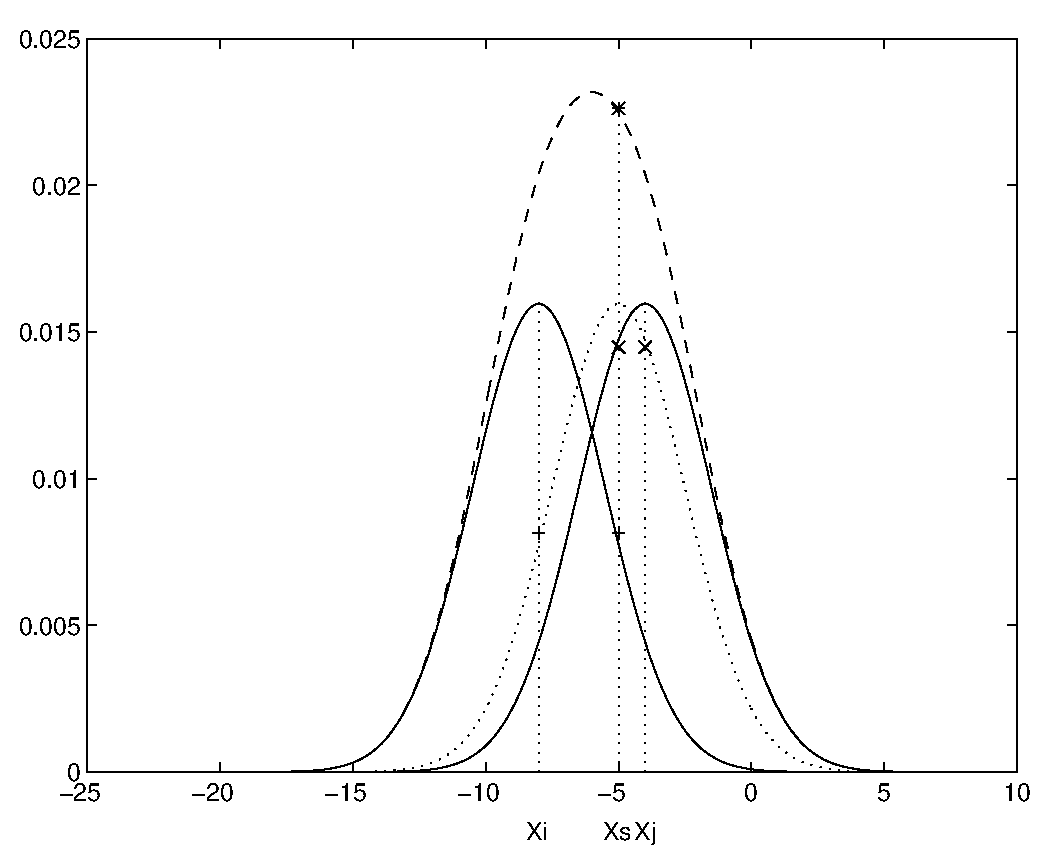
\includegraphics[height=6.2cm]{eijkel2}
\caption{One kernel at $x_s$ (\emph{dotted kernel}) or two kernels at
$x_i$ and $x_j$ (\textit{left and right}) lead to the same summed estimate
at $x_s$. This shows a figure consisting of different types of
lines. Elements of the figure described in the caption should be set in
italics, in parentheses, as shown in this sample caption.}
\label{fig:example}
\end{figure}

Please define figures (and tables) as floating objects. Please avoid
using optional location parameters like ``\verb+[h]+" for ``here".

\paragraph{Remark 1.}

In the printed volumes, illustrations are generally black and white
(halftones), and only in exceptional cases, and if the author is
prepared to cover the extra cost for color reproduction, are colored
pictures accepted. Colored pictures are welcome in the electronic
version free of charge. If you send colored figures that are to be
printed in black and white, please make sure that they really are
legible in black and white. Some colors as well as the contrast of
converted colors show up very poorly when printed in black and white.

\subsection{Formulas}

Displayed equations or formulas are centered and set on a separate
line (with an extra line or halfline space above and below). Displayed
expressions should be numbered for reference. The numbers should be
consecutive within each section or within the contribution,
with numbers enclosed in parentheses and set on the right margin --
which is the default if you use the \emph{equation} environment, e.g.,
\begin{equation}
  \psi (u) = \int_{o}^{T} \left[\frac{1}{2}
  \left(\Lambda_{o}^{-1} u,u\right) + N^{\ast} (-u)\right] dt \;  .
\end{equation}

Equations should be punctuated in the same way as ordinary
text but with a small space before the end punctuation mark.

\subsection{Footnotes}

The superscript numeral used to refer to a footnote appears in the text
either directly after the word to be discussed or -- in relation to a
phrase or a sentence -- following the punctuation sign (comma,
semicolon, or period). Footnotes should appear at the bottom of
the
normal text area, with a line of about 2~cm set
immediately above them.\footnote{The footnote numeral is set flush left
and the text follows with the usual word spacing.}

\subsection{Program Code}

Program listings or program commands in the text are normally set in
typewriter font, e.g., CMTT10 or Courier.

\medskip

\noindent
{\it Example of a Computer Program}
\begin{verbatim}
program Inflation (Output)
  {Assuming annual inflation rates of 7%, 8%, and 10%,...
   years};
   const
     MaxYears = 10;
   var
     Year: 0..MaxYears;
     Factor1, Factor2, Factor3: Real;
   begin
     Year := 0;
     Factor1 := 1.0; Factor2 := 1.0; Factor3 := 1.0;
     WriteLn('Year  7% 8% 10%'); WriteLn;
     repeat
       Year := Year + 1;
       Factor1 := Factor1 * 1.07;
       Factor2 := Factor2 * 1.08;
       Factor3 := Factor3 * 1.10;
       WriteLn(Year:5,Factor1:7:3,Factor2:7:3,Factor3:7:3)
     until Year = MaxYears
end.
\end{verbatim}
%
\noindent
{\small (Example from Jensen K., Wirth N. (1991) Pascal user manual and
report. Springer, New York)}

\subsection{Citations}

For citations in the text please use
square brackets and consecutive numbers: \cite{jour}, \cite{lncschap},
\cite{proceeding1} -- provided automatically
by \LaTeX 's \verb|\cite| \dots\verb|\bibitem| mechanism.

\subsection{Page Numbering and Running Heads}

There is no need to include page numbers. If your paper title is too
long to serve as a running head, it will be shortened. Your suggestion
as to how to shorten it would be most welcome.

\section{LNCS Online}

The online version of the volume will be available in LNCS Online.
Members of institutes subscribing to the Lecture Notes in Computer
Science series have access to all the pdfs of all the online
publications. Non-subscribers can only read as far as the abstracts. If
they try to go beyond this point, they are automatically asked, whether
they would like to order the pdf, and are given instructions as to how
to do so.

Please note that, if your email address is given in your paper,
it will also be included in the meta data of the online version.

\section{BibTeX Entries}

The correct BibTeX entries for the Lecture Notes in Computer Science
volumes can be found at the following Website shortly after the
publication of the book:
\url{http://www.informatik.uni-trier.de/~ley/db/journals/lncs.html}

\subsubsection*{Acknowledgments.} The heading should be treated as a
subsubsection heading and should not be assigned a number.

\section{The References Section}\label{references}

In order to permit cross referencing within LNCS-Online, and eventually
between different publishers and their online databases, LNCS will,
from now on, be standardizing the format of the references. This new
feature will increase the visibility of publications and facilitate
academic research considerably. Please base your references on the
examples below. References that don't adhere to this style will be
reformatted by Springer. You should therefore check your references
thoroughly when you receive the final pdf of your paper.
The reference section must be complete. You may not omit references.
Instructions as to where to find a fuller version of the references are
not permissible.

We only accept references written using the latin alphabet. If the title
of the book you are referring to is in Russian or Chinese, then please write
(in Russian) or (in Chinese) at the end of the transcript or translation
of the title.

The following section shows a sample reference list with entries for
journal articles \cite{jour}, an LNCS chapter \cite{lncschap}, a book
\cite{book}, proceedings without editors \cite{proceeding1} and
\cite{proceeding2}, as well as a URL \cite{url}.
Please note that proceedings published in LNCS are not cited with their
full titles, but with their acronyms!

\bibliographystyle{splncs03} 
\bibliography{refs}
\section*{Appendix: Springer-Author Discount}

LNCS authors are entitled to a 33.3\% discount off all Springer
publications. Before placing an order, the author should send an email, 
giving full details of his or her Springer publication,
to \url{orders-HD-individuals@springer.com} to obtain a so-called token. This token is a
number, which must be entered when placing an order via the Internet, in
order to obtain the discount.

\section{Checklist of Items to be Sent to Volume Editors}
Here is a checklist of everything the volume editor requires from you:


\begin{itemize}
\settowidth{\leftmargin}{{\Large$\square$}}\advance\leftmargin\labelsep
\itemsep8pt\relax
\renewcommand\labelitemi{{\lower1.5pt\hbox{\Large$\square$}}}

\item The final \LaTeX{} source files
\item A final PDF file
\item A copyright form, signed by one author on behalf of all of the
authors of the paper.
\item A readme giving the name and email address of the
corresponding author.
\end{itemize}
\end{document}
